\documentclass{beamer}

% opacity bugfix: see http://tug.org/pipermail/pdftex/2007-December/007480.html
\pdfpageattr {/Group << /S /Transparency /I true /CS /DeviceRGB>>}

\usepackage[utf8]{inputenc}
\usepackage[OT1]{fontenc}

\usepackage{tikz}
\usetikzlibrary{%
   arrows,%
   calc,%
   fit,%
   patterns,%
   plotmarks,%
   shapes.geometric,%
   shapes.misc,%
   shapes.symbols,%
   shapes.arrows,%
   shapes.callouts,%
   shapes.multipart,%
   shapes.gates.logic.US,%
   shapes.gates.logic.IEC,%
   er,%
   automata,%
   backgrounds,%
   chains,%
   topaths,%
   trees,%
   petri,%
   mindmap,%
   matrix,%
   calendar,%
   folding,%
   fadings,%
   through,%
   patterns,%
   positioning,%
   scopes,%
   decorations.fractals,%
   decorations.shapes,%
   decorations.text,%
   decorations.pathmorphing,%
   decorations.pathreplacing,%
   decorations.footprints,%
   decorations.markings,%
   shadows}
%\usepackage{animate}
\usepackage{amssymb, amsmath, amsfonts, enumerate}
\usepackage{eurosym}
\usepackage{pifont}
%\usepackage{bbold}
\newcommand\hmmax{0}
\usepackage{bm}
%\usepackage{dsfont}
\usepackage{pxfonts}
\usepackage{xcolor}
\usepackage{url}
\usepackage{xargs}

%\usepackage[backend=bibtex,style=authoryear,dashed=false]{biblatex}
%\addbibresource{../bib/lundrefs.bib}
%\renewcommand{\bibfont}{\normalfont\scriptsize}
%\setlength{\bibhang}{3ex}

\usepackage{hyperref}

\usetheme[official=false,department=none]{tue2008}
%\usefonttheme{default}


%\usetheme[secheader]{Boadilla}
%\setbeamercovered{transparent}
%\setbeamercovered{invisible}
%\setbeamertemplate{navigation symbols}{}
%\setbeamertemplate{bibliography item}[text] % numbered references
%\useoutertheme{infolines}
%\setbeamertemplate{headline}{}
%\setbeamertemplate{footline}{\hspace*{5mm}\hfill\insertframenumber\hspace*{5mm}\vspace{3mm}}
%\setbeamercolor{alerted text}{fg=orange!80!black}

% ------------------------------------------------------------------------------

\newcommand{\vcenterbox}[1]{\ensuremath{\vcenter{\hbox{#1}}}}
%
\newcommand{\reals}{\mathbb{R}}
\newcommand{\posreals}{\reals_{>0}}
\newcommand{\posrealszero}{\reals_{\ge 0}}
\newcommand{\naturals}{\mathbb{N}}

\newcommand{\dd}{\,\mathrm{d}}

\newcommand{\pr}{P}
\newcommand{\lpr}{\underline{P}}
\newcommand{\upr}{\overline{P}}
\newcommand{\lnex}{\underline{E}}
\newcommand{\unex}{\overline{E}}

\newcommand{\middlemid}{\;\middle\vert\;} % stretchable \mid
\newcommand{\prsymbol}{\operatorname{P}}
\newcommand{\lprsymbol}{\operatorname{\underline{P}}}
\newcommand{\uprsymbol}{\operatorname{\overline{P}}}
\newcommand{\expecsymbol}{\operatorname{E}}
\newcommand{\lexpecsymbol}{\operatorname{\underline{E}}}
\newcommand{\uexpecsymbol}{\operatorname{\overline{E}}}
\newcommand{\mediansymbol}{\operatorname{Median}}
\newcommand{\varsymbol}{\operatorname{Var}}
\newcommand{\sdsymbol}{\operatorname{SD}}
\newcommand{\covsymbol}{\operatorname{Cov}}
\newcommand{\pmfsymbol}{p}
\newcommand{\pdfsymbol}{f}
\newcommand{\cdfsymbol}{\operatorname{F}}
\newcommand{\risksymbol}{\rho}
\newcommand{\helper}[3]{
  \ifthenelse{\equal{#3}{}}{%
    {#1}_{#2}}{%
    {#1}_{#2}\left({#3}\right)}{%
  }
}
%\newcommand{\pr}[2][]{\helper{\prsymbol}{#1}{#2}}
%\newcommand{\lpr}[2][]{\helper{\lprsymbol}{#1}{#2}}
%\newcommand{\upr}[2][]{\helper{\uprsymbol}{#1}{#2}}
\newcommand{\expec}[2][]{\helper{\expecsymbol}{#1}{#2}}
\newcommand{\median}[2][]{\helper{\mediansymbol}{#1}{#2}}
\newcommand{\var}[2][]{\helper{\varsymbol}{#1}{#2}}
%\newcommand{\sd}[2][]{\helper{\sdsymbol}{#1}{#2}}
\newcommand{\cov}[2][]{\helper{\covsymbol}{#1}{#2}}
\newcommand{\risk}[2][]{\helper{\risksymbol}{#1}{#2}}
\newcommand{\pmf}[2][]{\helper{\pmfsymbol}{#1}{#2}}
\newcommand{\pdf}[2][]{\helper{\pdfsymbol}{#1}{#2}}
\newcommand{\cdf}[2][]{\helper{\cdfsymbol}{#1}{#2}}
\newcommand{\chelper}[5]{
  \ifthenelse{\equal{#3}{}}{%
    {#1}_{#2}\left(#4 \middlemid #5 \right)}{%
    {#1}_{#2\mid #3}\left(#4 \middlemid #5 \right)}{%
  }
}
\newcommand{\cpr}[2]{\chelper{\prsymbol}{}{}{#1}{#2}}
\newcommand{\clpr}[2]{\chelper{\lprsymbol}{}{}{#1}{#2}}
\newcommand{\cupr}[2]{\chelper{\uprsymbol}{}{}{#1}{#2}}
\newcommand{\cexpec}[2]{\chelper{\expecsymbol}{}{}{#1}{#2}}
\newcommand{\clexpec}[2]{\chelper{\lexpecsymbol}{}{}{#1}{#2}}
\newcommand{\cuexpec}[2]{\chelper{\uexpecsymbol}{}{}{#1}{#2}}
\newcommand{\cmedian}[2]{\chelper{\mediansymbol}{}{}{#1}{#2}}
\newcommand{\cvar}[2]{\chelper{\varsymbol}{}{}{#1}{#2}}
\newcommand{\ccov}[2]{\chelper{\covsymbol}{}{}{#1}{#2}}
\newcommand{\csd}[2]{\chelper{\sdsymbol}{}{}{#1}{#2}}
\newcommand{\crisk}[2]{\chelper{\risksymbol}{}{}{#1}{#2}}
\newcommandx{\cpmf}[4][1=,2=]{\chelper{\pmfsymbol}{#1}{#2}{#3}{#4}}
\newcommandx{\cpdf}[4][1=,2=]{\chelper{\pdfsymbol}{#1}{#2}{#3}{#4}}
\newcommandx{\ccdf}[4][1=,2=]{\chelper{\cdfsymbol}{#1}{#2}{#3}{#4}}

\newcommand{\mbf}[1]{\mathbf{#1}}
\newcommand{\bs}[1]{\boldsymbol{#1}}
\renewcommand{\vec}[1]{{\bm#1}}

\newcommand{\uz}{^{(0)}} % upper zero
\newcommand{\un}{^{(n)}} % upper n
\newcommand{\ui}{^{(i)}} % upper i
\newcommand{\uell}{^{(\ell)}} % upper ell

\newcommand{\ul}[1]{\underline{#1}}
\newcommand{\ol}[1]{\overline{#1}}

\newcommand{\Rsys}{R_\text{sys}}
\newcommand{\lRsys}{\ul{R}_\text{sys}}
\newcommand{\uRsys}{\ol{R}_\text{sys}}

\newcommand{\Fsys}{F_\text{sys}}
\newcommand{\lFsys}{\ul{F}_\text{sys}}
\newcommand{\uFsys}{\ol{F}_\text{sys}}

\def\Tsys{T_\text{sys}}

\newcommand{\E}{\operatorname{E}}
\newcommand{\V}{\operatorname{Var}}
\newcommand{\sd}{\operatorname{sd}}

\newcommand{\wei}{\operatorname{Wei}} % Weibull Distribution
\newcommand{\ig}{\operatorname{IG}}   % Inverse Gamma Distribution
\newcommand{\ber}{\operatorname{Bernoulli}} 
\newcommand{\bin}{\operatorname{Binomial}}
\newcommand{\be}{\operatorname{Beta}} 
\newcommand{\bebin}{\operatorname{Beta-binomial}}
\newcommand{\norm}{\operatorname{N}}

\newcommand{\then}{\structure{$\rule[0.35ex]{2ex}{0.5ex}\!\!\!\blacktriangleright$}}
\newcommand{\play}{\structure{$\blacktriangleright$}}
%\newcommand{\gplus}{\structure{\rule[0.45ex]{1.4ex}{0.4ex}\hspace{-0.9ex}\rule[0.0ex]{0.4ex}{1.3ex}\hspace{0.5ex}}}
\newcommand{\gplus}{\structure{\textbf{+}}}
%\newcommand{\gmins}{\structure{\rule[0.45ex]{1.4ex}{0.4ex}}}
\newcommand{\gmins}{\structure{\textbf{--}}}
\newcommand{\gexcl}{\structure{\rule{0.3ex}{0ex}\textbf{!}\rule{0.3ex}{0ex}}}


\def\yz{y\uz}
\def\yn{y\un}
%\def\yi{y\ui}
\newcommand{\yfun}[1]{y^{({#1})}}
\newcommand{\yfunl}[1]{\ul{y}^{({#1})}}
\newcommand{\yfunu}[1]{\ol{y}^{({#1})}}

\def\ykt{y_{k,t}}

\def\ykz{y\uz_k}
\def\ykn{y\un_k}

\def\yktz{y\uz_{k,t}}
\def\yktn{y\un_{k,t}}

\def\yzl{\ul{y}\uz}
\def\yzu{\ol{y}\uz}
\def\ynl{\ul{y}\un}
\def\ynu{\ol{y}\un}
\def\yil{\ul{y}\ui}
\def\yiu{\ol{y}\ui}

\def\ykzl{\ul{y}\uz_k}
\def\ykzu{\ol{y}\uz_k}
\def\yknl{\ul{y}\un_k}
\def\yknu{\ol{y}\un_k}

\def\yktzl{\ul{y}\uz_{k,t}}
\def\yktzu{\ol{y}\uz_{k,t}}
\def\yktnl{\ul{y}\un_{k,t}}
\def\yktnu{\ol{y}\un_{k,t}}


\def\nz{n\uz}
\def\nn{n\un}
%\def\ni{n\ui}
\newcommand{\nfun}[1]{n^{({#1})}}
\newcommand{\nfunl}[1]{\ul{n}^{({#1})}}
\newcommand{\nfunu}[1]{\ol{n}^{({#1})}}

\def\nkz{n\uz_k}
\def\nkn{n\un_k}
\newcommand{\nkzfun}[1]{n\uz_{#1}}

\def\nkt{n_{k,t}}

\def\nktz{n\uz_{k,t}}
\def\nktn{n\un_{k,t}}


\def\nzl{\ul{n}\uz}
\def\nzu{\ol{n}\uz}
\def\nnl{\ul{n}\un}
\def\nnu{\ol{n}\un}
\def\nil{\ul{n}\ui}
\def\niu{\ol{n}\ui}

\def\nkzl{\ul{n}\uz_k}
\def\nkzu{\ol{n}\uz_k}
\def\nknl{\ul{n}\un_k}
\def\nknu{\ol{n}\un_k}

\def\nktzl{\ul{n}\uz_{k,t}}
\def\nktzu{\ol{n}\uz_{k,t}}
\def\nktnl{\ul{n}\un_{k,t}}
\def\nktnu{\ol{n}\un_{k,t}}

\def\taut{\tau(\vec{t})}
\def\taux{\tau(\vec{x})}
\def\ttau{\tilde{\tau}}
\def\ttaut{\ttau(\vec{t})}
\def\ttaux{\ttau(\vec{x})}

\def\MZ{\mathcal{M}\uz}
\def\MN{\mathcal{M}\un}

\def\MkZ{\mathcal{M}\uz_k}
\def\MkN{\mathcal{M}\un_k}

\def\MktZ{\mathcal{M}\uz_{k,t}}
\def\MktN{\mathcal{M}\un_{k,t}}

\def\PZ{\Pi\uz}
\def\PN{\Pi\un}

\def\PkZ{\Pi\uz_k}
\def\PkN{\Pi\un_k}
\newcommand{\PZi}[1]{\Pi\uz_{#1}}

\def\PktZ{\Pi\uz_{k,t}}
\def\PktN{\Pi\un_{k,t}}
\newcommand{\PtZi}[1]{\Pi\uz_{#1,t}}
\newcommand{\PkZi}[1]{\Pi\uz_{k,#1}}

\newcommand{\az}{\alpha\uz}
\newcommand{\an}{\alpha\un}
\newcommand{\bz}{\beta\uz}
\newcommand{\bn}{\beta\un}


\def\blau#1{{\color{tuegreen}#1}}
\def\rot#1{{\color{tuered}#1}}
\def\gruen#1{{\color{tueblue}#1}}

\def\yzr{\rot{\yz}}
\def\ynr{\rot{\yn}}
\def\byzr{\rot{\byz}}
\def\bynr{\rot{\byn}}
\def\yzor{\rot{y\uz_1}}
\def\yzjr{\rot{y\uz_j}}
\def\yzkr{\rot{y\uz_k}}
\def\yzlr{\rot{\yzl}}
\def\yzur{\rot{\yzu}}
\def\ynjr{\rot{y\un_j}}
\def\ynlr{\rot{\ynl}}
\def\ynur{\rot{\ynu}}
\def\yzjlr#1{\rot{\ul{y}\uz_#1}}
\def\yzjur#1{\rot{\ol{y}\uz_#1}}

\def\yktzr{\rot{\yktz}}
\def\yktnr{\rot{\yktn}}

\def\nzg{\gruen{\nz}}
\def\nng{\gruen{\nn}}
\def\nzlg{\gruen{\nzl}}
\def\nzug{\gruen{\nzu}}
\def\nnlg{\gruen{\nnl}}
\def\nnug{\gruen{\nnu}}
\def\nzjlg#1{\gruen{\ul{n}\uz_#1}}
\def\nzjug#1{\gruen{\ol{n}\uz_#1}}

\def\nktzg{\gruen{\nktz}}
\def\nktng{\gruen{\nktn}}

\def\psib{\blau{\psi}}
\def\bpsib{\blau{{b}(\psi)}}


% ------------ shading start
\newsavebox{\tempbox}
\newcommand\leftrightshading[3]{%
  \begin{tikzfadingfrompicture}[name=inputtext]
    \node [text=white] {#1};
  \end{tikzfadingfrompicture}
  \begin{lrbox}{\tempbox}%
    \begin{tikzpicture}
      \node [text=white,inner sep=0pt,outer sep=0pt] (textnode) {#1};
      \shade[path fading=inputtext,fit fading=false,left color=#2,right color=#3]
      (textnode.south west) rectangle (textnode.north east);
    \end{tikzpicture}%
  \end{lrbox}
  % Now we use the fading in another picture:
  \usebox\tempbox{}%
}
% ------------ shading end


%\def\PZc{\mathrm I\!\Pi\uz}
\def\PZc{\leftrightshading{$\mathrm I\!\Pi\uz$}{blue}{red}}
\def\PktZc{\leftrightshading{${\mathrm I\!\Pi_{k,t}\uz}$}{blue}{red}}
%\def\PNc{\PN}
\def\PNc{\leftrightshading{$\mathrm I\!\Pi\un$}{blue}{red}}



%%\def\blau#1{{\color{lmugreen2}#1}}
%\def\rot#1{{\color{red}#1}}
%\def\gruen#1{{\color{blue}#1}}

\newcommand{\x}{\vec{x}}

\def\tnow{t_\text{now}}
\def\tpnow{t^+_\text{now}}

\newcommand{\comp}[1]{\raisebox{-1mm}{\tikz{\node[%type1
rectangle,rounded corners=0mm,draw,fill=tuepmsgreen!70,thick,inner sep=0pt,minimum size=4mm]{#1};}}}

\newcommand{\cyansec}[1]{\textcolor{tuecyan}{\large\bf #1}}
\newcommand{\cyanalert}[1]{\textcolor{tuecyan}{#1}}
\newcommand{\bluesec}[1]{\textcolor{tueblue}{\large\bf #1}}
\newcommand{\bluealert}[1]{\textcolor{tueblue}{#1}}

\setbeamertemplate{itemize item}{\tiny\raise1.5pt\hbox{\color{tueblue}$\blacktriangleright$}}

% ------------------------------------------------------------------------------


\title{Imprecise Probability:\\ General Ideas and Statistical Approaches}

\author{Gero Walter}
\institute{ Eindhoven University of Technology, Eindhoven, NL\\[2ex]
            \url{g.m.walter@tue.nl} \\[2ex]
            
\includegraphics[height=9mm]{logos/tuelogo} \\[2ex] %\quad
            %
\includegraphics[height=9mm]{logos/dinalog-hp} }
            Thanks to Matthias Troffaes for introductory slides.}
\date{Hannover 2016-12-07}

\begin{document}

\frame{
\titlepage
}

\addtocounter{framenumber}{-1} 

\begin{frame}
  \frametitle{Requirements for an Uncertainty Model}
  \begin{block}{Operational}
    How can uncertainty be reliably
    \begin{itemize}
    \item measured?
    \item communicated?
    \end{itemize}
  \end{block}
  \begin{block}{Inference}
    How can we use our theory of uncertainty for
    \begin{itemize}
    \item statistical reasoning?
    \item decision making?
    \end{itemize}
  \end{block}
\end{frame}

\begin{frame}
  \frametitle{Uncertainty via Probability}
  \begin{definition}
    An \alert{event} is a statement that may, or may not,
    hold \\
    ---typically, something that may happen in the future.
    \\[1ex]
    Notation: $A$, $B$, $C$, \dots
  \end{definition}
  \begin{exampleblock}{Examples}
    \begin{itemize}
    \item tomorrow, it will rain
    \item in the next year, at most 3 components will fail
    \end{itemize}
  \end{exampleblock}
  \begin{alertblock}{}
    how to express our uncertainty regarding events?
  \end{alertblock}
\end{frame}

\begin{frame}
  \frametitle{Probability: Definition}
  \begin{definition}
    The \alert{probability of an event} is a number between $0$ and $1$.
    \\[1ex]
    Notation: $P(A)$, $P(B)$, $P(C)$, \dots
  \end{definition}
  \begin{exampleblock}{Examples}
    \begin{itemize}
    \item for $A$ = `tomorrow, it will rain' \\
      my probability $P(A)$ is $0.2$
    \item for $B$ = `in the next year, at most 3 components will fail' \\
      my probability $P(B)$ is $0.0173$
    \end{itemize}
  \end{exampleblock}
  \begin{alertblock}{}
    what do these numbers actually mean? \\
    how would you measure them?
  \end{alertblock}
\end{frame}

\begin{frame}
  \frametitle{Probability: Interpretation}
  \begin{block}{Interpretation: Trivial Cases}
    $P(A)=0$ $\iff$ $A$ is practically impossible {\hfill \scriptsize logically?}\\
    $P(A)=1$ $\iff$ $A$ is practically certain
  \end{block}
  \begin{alertblock}{}
    what about values between $0$ and $1$, such as $P(A)=0.2$?
  \end{alertblock}
  \begin{block}{Interpretation: General Case}
    \begin{itemize}
    \item it's (like) a \alert{frequency}
    \item it's a degree of belief (\play\ \alert{betting rate})
    \item it's something else
    \end{itemize}
  \end{block}
\end{frame}

\begin{frame}
  \frametitle{Probability: Frequency Interpretation}
  $P(A)=0.2$ means:
  \begin{itemize}
  \item in 1 out of 5 times, it rains tomorrow \\
    \textbf{??? (tomorrow is not repeatable!)}
  \item on a `day like this', in 1 out of 5 times, it rains the next day
  \end{itemize}
  \begin{block}{Frequency Interpretation}
    \begin{itemize}
    \item[\gplus] intuitive, easy to understand
    \item[\gmins] needs \alert{reference class}, only for \alert{repeatable events}
    \item[\gmins] needs plenty of data, or strong symmetry assumptions
    \item[\gexcl] aleatory
    \end{itemize}
  \end{block}
\end{frame}

\begin{frame}
  \frametitle{Probability: Betting Interpretation}
  $P(A)=0.2$ means:
  \begin{itemize}
  \item I would \textit{now} pay at most \euro 0.2 \\
    if \textit{tomorrow} I am paid \euro 1 in case it rains
  \item I would \textit{tomorrow} pay \euro 1 in case it rains \\
    if I am \textit{now} paid at least \euro 0.2
  \end{itemize}
  \begin{center}
    \begin{tikzpicture}
      \draw (-4,0) -- (4,0);
      \draw[line width=1mm,tuegreen] (-4,0) -- (0,0);
      \draw[line width=1mm,tueblue]  ( 0,0) -- (4,0);
      \draw ( 0,-0.1) -- ( 0,0.1) node[above] {$P(A)$};
      \draw[dashed] ( 0,0) -- (0,-0.5);
      \draw (-2,0.1) node[above] {$p$} -- (-2,-0.1) node[anchor=north east,xshift=1cm] {buy $A$ for price $p$};
      \draw ( 2,0.1) node[above] {$q$} -- ( 2,-0.1) node[anchor=north west,xshift=-1cm] {sell $A$ for price $q$};
    \end{tikzpicture}
  \end{center}
  \vspace*{-1.5ex}
  \begin{block}{Betting (Degree of Belief) Interpretation}
    \begin{itemize}
    \item[\gplus] no reference class, works also for \alert{one-shot events}
    \item[\gmins] needs plenty of elicitation or plenty of data
    \item[\gexcl] epistemic
    \end{itemize}
  \end{block}
\end{frame}

\begin{frame}
  \frametitle{Dealing With Severe Uncertainty}
  \begin{alertblock}{}
    in case of \alert{partial elicitation} and/or \alert{sparse data}
    \\
    it may be hard to specify an exact probability
    \\
    \textbf{but you may still confidently bound your probability}
  \end{alertblock}
  \vspace{2em}
  this becomes more and more relevant \\
  as problems become larger and larger
\end{frame}

\begin{frame}
  \frametitle{Bounding Methods} %\normalsize Dealing With Severe Uncertainty: 
%  \begin{columns}
%  \begin{column}{\textwidth}
%  \begin{block}{Confidence intervals} %[]
\structure{Confidence intervals (Frequentist Statistics)}
    \begin{itemize}
  \setlength{\itemsep}{0pt}
  \setlength{\parskip}{0pt}
  \setlength{\parsep}{0pt}
    \item[\gmins] choice of confidence level $\alpha$?
    \item[\gmins] p-value fallacy (aka prosecutor's fallacy)
    \item[\gplus] no prior needed, only likelihood
    \end{itemize}
%  \end{block}
  \vspace*{1ex}
%  \begin{block}{Credible intervals}
\structure{Credible intervals (Bayesian Statistics)}
      \begin{itemize}
  \setlength{\itemsep}{0pt}
  \setlength{\parskip}{0pt}
  \setlength{\parsep}{0pt}
      \item[\gmins] choice of credible level $\alpha$?
      \item[\gmins] choice of prior?
      \item[\gmins] dealing with prior ignorance and prior-data conflict?
      \item[\gplus] no p-value fallacy
      \end{itemize}
%  \end{block}
%  \end{column}
%  \end{columns}
%  \begin{columns}
%  \begin{column}{0.8\textwidth}
  \vspace*{1ex}
%  \begin{block}{Interval probability (bounding probabilities directly)}
\structure{Interval probability (bounding probabilities directly)}
    \begin{itemize}
  \setlength{\itemsep}{0pt}
  \setlength{\parskip}{0pt}
  \setlength{\parsep}{0pt}
    \item[\gmins] choice of prior bounds?
    \item[\gplus] no confidence / credible level issues
    \item[\gplus] no prior ignorance issues
    \item[\gplus] no p-value fallacy
    \end{itemize}
%  \end{block}
%  \end{column}
%  \begin{column}{0.2\textwidth}
%  \end{column}
%  \end{columns}
%  {\scriptsize other: info-gap \cite{2001:benhaim}, \dots}
\end{frame}

\begin{frame}
  \frametitle{Lower and Upper Probability: Definition}
  \begin{definition}
    The \alert{lower and upper probability of an event}\\ are numbers between $0$ and $1$.
    \\[1ex]
    Notation: $\lpr(A)$, $\upr(A)$, \dots
  \end{definition}
  \begin{exampleblock}{Examples}
    \begin{itemize}
    \item for $A$ = `tomorrow, it will rain' \\
      my lower probability $\lpr(A)$ is $0.1$ \\
      my upper probability $\upr(A)$ is $0.4$
    \end{itemize}
  \end{exampleblock}
  \begin{alertblock}{}
    what do these numbers actually mean? \\
    how would you measure them?
  \end{alertblock}
\end{frame}

\begin{frame}
  \frametitle{$\lpr$ and $\upr$: Betting Interpretation}
  $\lpr(A)=0.1$ and $\upr(A)=0.4$ means:
  \begin{itemize}
  \item I would \textit{now} pay at most \euro 0.1 \\
    if \textit{tomorrow} I am paid \euro 1 in case it rains
  \item I would \textit{tomorrow} pay \euro 1 in case it rains \\
    if I am \textit{now} paid at least \euro 0.4
  \end{itemize}
  \vspace*{-3ex}
  \begin{center}
    \begin{tikzpicture}
      \draw (-4,0) -- (4,0);
      \draw[line width=1mm,tuegreen] (-4,0) -- (-1,0);
      \draw[line width=1mm,tueblue] (1,0) -- (4,0);
      \draw[line width=1mm,tueorange] (-1,0) -- (1,0);
      \draw (-1,-0.1) -- (-1,0.1) node[above] {$\lpr(A)$};
      \draw[dashed] (-1,0) -- (-1,-0.5);
      \draw ( 1,-0.1) -- ( 1,0.1) node[above] {$\upr(A)$};
      \draw[dashed] ( 1,0) -- ( 1,-0.5);
      \draw (0,-0.1) node[below] {\small \textcolor{tueorange}{undecisive}};
      \draw (-2,0.1) node[above] {$p$} -- (-2,-0.1) node[anchor=north east,xshift= 0.8cm] {\small buy $A$ for price $p$};
      \draw ( 2,0.1) node[above] {$q$} -- ( 2,-0.1) node[anchor=north west,xshift=-0.8cm] {\small sell $A$ for price $q$};
    \end{tikzpicture}
  \end{center}
\vspace*{-1ex}
  \begin{block}{Betting Interpretation}
    \begin{itemize}
    \item[\gplus] no reference class, works also for \alert{one-shot events}
    \item[\gplus] works with partial elicitation and / or sparse data
    \item[\gexcl] epistemic
    \end{itemize}
  \end{block}
%  {\scriptsize \qquad frequency interpretation?}
\end{frame}

\begin{frame}
  \frametitle{Events: Formal Definition}
  \begin{definition}
    The \alert{possibility space} $\Omega$ is \\
    the set of all possible outcomes of the problem at hand.
  \end{definition}
  \vspace*{-1ex}
  \begin{exampleblock}{Example}
    interested in reliability of a system with $5$ components \\
    e.g. number of components that fail in the next year \\
    $\Omega=\{0,1,2,3,4,5\}$
  \end{exampleblock}
  \begin{definition}
    An \alert{event} is a subset of $\Omega$.
    %\\[1ex]
    \hspace{2em}
    Notation: $A$, $B$, $C$, \dots
  \end{definition} 
  \vspace*{-1ex}
  \begin{exampleblock}{Example}
    in the next year, at most 3 components will fail
    \\
    would be represented by the event $A=\{0,1,2,3\}$
  \end{exampleblock}
\end{frame}

\begin{frame}
  \frametitle{$\lpr$ and $\upr$: Formal Definition}
  \begin{definition}
    A \alert{lower probability} $\lpr$
    \\
    maps
    \textit{every}
    event $A\subseteq\Omega$ to a real number $\lpr(A)$.
    \\[1ex]
    The \alert{upper probability} $\upr$ is simply defined as \\
    $\upr(A)=1-\lpr(A^c)$, for all $A\subseteq\Omega$
  \end{definition}
  \begin{itemize}
  \item $A^c$ = \alert{complement} (or \alert{negation}) of $A$ = all elements {\it not} in $A$
  \begin{exampleblock}{Example}
    complement of `at most 3 components will fail' ($A=\{0,1,2,3\}$)
    \\ is `at least 4 components will fail' ($A^c=\{4,5\}$)
  \end{exampleblock}
  \item {\small the identity $\upr(A)=1-\lpr(A^c)$ is implied
    by the betting interpretation }%\\
%    {\scriptsize \hfill see exercises}
  \item {\small \textit{every} event $\leftrightarrow$ sparse data? \\
    we can always set $\lpr(A)=0$ and $\lpr(A^c)=0$ ($\iff\upr(A)=1$)!}
  \end{itemize}
\end{frame}

\begin{frame}
  \frametitle{$\lpr$ and $\upr$: Credal Sets}
  \begin{definition}
    A \alert{probability measure} $\pr$
    \\
    maps
    \textit{every}
    event $A\subseteq\Omega$ to a number $\pr(A)$
    in $[0,1]$
    and satisfies
\begin{columns}
\begin{column}{0.2\textwidth}
    \begin{itemize}
    \item $\pr(\emptyset)=0$,
    \end{itemize}
\end{column}
\begin{column}{0.3\textwidth}
    \begin{itemize}
    \item $\pr(\Omega)=1$, and
    \end{itemize}
\end{column}
\begin{column}{0.45\textwidth}
    \begin{itemize}
    \item $\pr(A)=\sum_{\omega\in A}\pr(\{\omega\})$.
    \end{itemize}
\end{column}
\end{columns}
  \end{definition}
  \begin{definition}
    The \alert{credal set} $\mathcal{M}$
    of $\lpr$
    \\ is the set of all probability measures $\pr$ for which
    \\ 
    $\lpr(A)\le\pr(A)\le\upr(A)$ for all $A\subseteq\Omega$.
  \end{definition}
  \begin{block}{Sensitivity Interpretation of $\lpr$}
    One of the probability measures $\pr$ in the credal set $\mathcal{M}$\\
    is the correct one,
    \textit{but we do not know which}.
  \end{block}
%  \begin{center}
    \textbf{crucial: no distribution over $\mathcal{M}$ assumed!} %\\
%    (why not?)
%  \end{center}
\end{frame}

\iffalse
\begin{frame}
  \frametitle{$\lpr(\cdot)$ and $\upr(\cdot)$:
%    Avoiding Sure Loss, Natural Extension, and Coherence}
     Properties***}
  \begin{definition}
    We say that $\lpr$ \alert{avoid sure loss} if its credal set $\mathcal{M}$ is non-empty.
  \end{definition}
  \begin{definition}
    If $\lpr$ avoids sure loss, its \alert{natural extension} $\lnex$ is defined, for all $A\subseteq\Omega$, as:
    \begin{align*}
      \lnex(A)=\min_{\pr\in\mathcal{M}}\pr(A)
      &&
      \left(\text{or equivalently, }\unex(A)=\max_{\pr\in\mathcal{M}}\pr(A)\right)
    \end{align*}
  \end{definition}
  \begin{definition}
    We say that $\lpr$ is \alert{coherent} if it avoids sure loss, and, for all $A\subseteq\Omega$:
    \begin{align*}
      \lpr(A)=\lnex(A)
      &&
      \Big(\text{or equivalently, }\upr(A)=\unex(A)\Big)
    \end{align*}
  \end{definition}
\end{frame}

\begin{frame}
  \frametitle{$\lpr(\cdot)$ and $\upr(\cdot)$: Sensitivity Interpretation}
  \begin{block}{Sensitivity Interpretation of $\lpr$}
    One of the probability measures $\pr$ in the credal set $\mathcal{M}$ is
    the correct one,
    \textit{but we do not know which}.
  \end{block}
%  \begin{itemize}
%  \item $\lpr$ is coherent precisely when it is
%    \\ \alert{uniquely determined} by $\mathcal{M}$
%  \item if $\lpr$ is not coherent, but avoids sure loss
%    \\
%    then its natural extension $\lnex$ \alert{corrects} $\lpr$
%  \end{itemize}
  \begin{center}
    \textbf{crucial: no distribution over $\mathcal{M}$ assumed!} %\\
%    (why not?)
  \end{center}
\end{frame}
\fi

\begin{frame}{Bayesian Inference}
\vspace*{-2ex}
\begin{align*}
\begin{array}{ccccl}
\uncover<1->{\text{expert info}        & + & \text{data}                & \to & \text{complete picture} \\[1.5ex]}
\uncover<2->{\text{prior distribution} & + & \text{sample distribution} & \to & \text{posterior distribution} \\[1.5ex]
 f(p) & \times & f(s \mid p) & \propto & f(p \mid s) \\
 & & & & \qquad\text{\bluealert{\play\ Bayes' Rule}} \\}
%\uncover<3->{\downarrow & & \downarrow & & \hspace*{3ex} \downarrow \\
\uncover<4->{\text{Beta prior}}   & & \uncover<3->{\text{Binomial}}         & & \uncover<5->{\text{Beta posterior}} \\
\uncover<4->{}                    & & \uncover<3->{\text{distribution}}     & & \uncover<5->{\qquad \text{\bluealert{\play\ conjugacy}}}\\[1ex]
\uncover<4->{p \sim \be(\az,\bz)} & & \uncover<3->{s \mid p \sim \bin(n,p)} & & \uncover<5->{p \mid s \sim \be(\an,\bn)}
\end{array}
\end{align*}
\vspace*{-3ex}
\begin{tikzpicture}
\uncover<3-5>{%
\node at (-0.5,0) {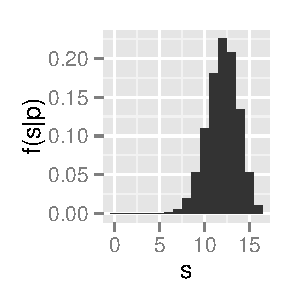
\includegraphics[width=0.25\textwidth]{figs/smallfig-binom}};}
\uncover<4-5>{%
\node at (-4.5,0) {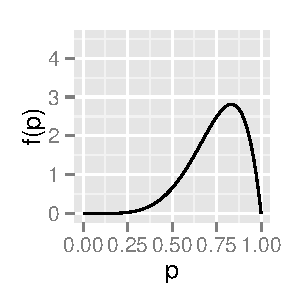
\includegraphics[width=0.25\textwidth]{figs/smallfig-prior}};}
\uncover<5>{%
\node at ( 3.5,0) {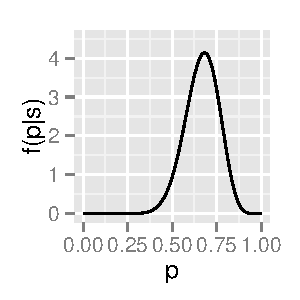
\includegraphics[width=0.25\textwidth]{figs/smallfig-posterior}};}
\end{tikzpicture}
\end{frame}

\begin{frame}{Bayesian Inference with Sets of Priors}
Bayesian inference with sets of priors (credal sets):\\ \emph{robust Bayesian inference}
\begin{itemize}
\item prior ignorance / weakly informative priors
\item prior-data conflict
\end{itemize}
***make noninformative prior thing short
\end{frame}

\begin{frame}{`Non-informative' Priors}
  How to construct a prior if we do not have a lot of information?
  \begin{alertblock}{Laplace: Principle of Indifference}
    Use the uniform distribution.
  \end{alertblock}
  Obvious issue: this depends on the parametrisation!
%  \pause
  \begin{exampleblock}{Example}
    An object of 1kg has uncertain volume $V$ between $1\ell$ and $2\ell$.
    \begin{itemize}
    \item Uniform distribution over volume $V$ $\implies$ $E(V)=1.5\ell$.
    \item Uniform distribution over density $\rho=1/V$ $\implies$ \\
      $E(V)=E(1/\rho)=\int_{0.5}^1 2/\rho d\rho=2(\ln 1-\ln 0.5)=1.39\ell$
    \end{itemize}
  \end{exampleblock}
%  \pause
  \alert{The uniform distribution does not really model prior ignorance.}
  (Jeffreys prior is transformation-invariant, but depends on the sample space and can break decision making!)
\end{frame}

\begin{frame}{Prior Ignorance via Sets of Probabilities}
   How to construct prior if we do not have a lot of information?
  \begin{alertblock}{Boole: Probability Bounding}
    Use the set of all probability distributions (\alert{vacuous model}).
  \end{alertblock}
  Results no longer depend on parametrisation!
%  \pause
  \begin{exampleblock}{Example}
    An object of 1kg has uncertain volume $V$ between $1\ell$ and $2\ell$.
    \begin{itemize}
    \item Set of all distributions over volume $V$ $\implies$ $E(V)\in[1,2]$.
    \item Set of all distribution over density $\rho=1/V$ $\implies$ \\
      $E(V)=E(1/\rho)\in[1,2]$
    \end{itemize}
  \end{exampleblock}
\end{frame}

\begin{frame}{Prior Ignorance via Sets of Probabilities}
  \begin{theorem}
    The set of posterior distributions
    resulting from a vacuous set of prior distributions
    is again vacuous,
    regardless of the likelihood.
  \end{theorem}
  \alert{We can never learn anything when starting from a vacuous set of priors.}
  \pause
  \begin{alertblock}{Solution: Near-Vacuous Sets of Priors}
    Only insist that the prior predictive, or other classes of inferences, are vacuous.
  \end{alertblock}
  This can be done using sets of conjugate priors ***%\cite{2012:benavolizaffalon,2015:benavolizaffalon}.
\end{frame}


\begin{frame}{Example: Imprecise Beta Model (IBM)}
***use other BBM intro slides?
\begin{itemize}
\item<1-> binomial likelihood (observing $x$ successes in $n$ trials)
\begin{align*}
\cpdf{x}{\theta} &= {n \choose x} \, \theta^x (1-\theta)^{n-x}
\end{align*}
\item<1-> conjugate Beta prior
      \begin{itemize} 
      \item with mean $\yzr$
        = prior expected probability of success
      \item and prior strength parameter $\nzg>0$
      \end{itemize}
\begin{align*}
\pdf{\theta} &\propto \theta^{\nzg\yzr-1}\, (1-\theta)^{\nzg(1-\yzr)-1}
\end{align*}
\item<2-> ***informative set of priors: Use the set $\MZ$ of Beta priors with $\yzr \in [\yzlr, \yzur]$ and
      \begin{itemize} 
      \item $\nzg > 0$ fixed, or
      \item $\nzg \in [\nzlg, \nzug]$
      \end{itemize}
\item<3-> $\cexpec{\theta}{x} = \ynr$ is a weighted average of $\expec{\theta} = \yzr$ and $\dfrac{x}{n}$!
\item<4-> $\cvar{\theta}{x} = \dfrac{\ynr (1-\ynr)}{\nng + 1}$ decreases with $n$!
\end{itemize}
%($\theta_1 \to \theta$, $\theta_2 \to 1-\theta$, $t_1 \to \yzr$, $t_2 = 1 - t_1$, $n_1 = x$, $n_2 = n-x$, $s \to \nzg$)
\end{frame}

\begin{frame}{}
***do the whole param update thing, also near-noninf, like lund (?)
\end{frame}



\begin{frame}{%General Framework for 
Canonical Exponential Families}
  Conjugate priors like the Beta can be constructed
  for sample distributions (likelihood) from:
  \begin{definition}[Canonical exponential family]
  \begin{equation*}
    f(x \mid \psi)=h(x)\exp\big\{\psib^T\tau(x) - \bpsib) \big\}
  \end{equation*}
  \begin{itemize}
  \item includes multinomial, normal, Poisson, exponential, \dots
  \item $\psi$ generally a transformation of original parameter $\theta$
  \end{itemize}
  \pause
  \end{definition}
  \begin{definition}[Family of conjugate priors]
  A family of priors for i.i.d.\ sampling from the can.\ exp.\ family:
  \begin{equation*}
    f(\psib\mid\nzg,\yzr)
    \propto \exp\big\{ \nzg \big[\psib^T \yzr - \bpsib\big]\big\}
  \end{equation*}
  with hyper-parameters $\nzg$ and $\yzr$.
  \end{definition}
\end{frame}

\begin{frame}
    \end{equation*}
    where
    \begin{align*}
      \vec{x} &= (x_1,\dots,x_n) &
      \tau(\vec{x}) &= \sum_{i=1}^n \tau(x_i) \\
      \nng &= \nzg + n &
      \ynr &= \frac{\nzg}{\nzg + n} \cdot \yzr + \frac{n}{\nzg + n} \cdot \frac{\tau(\vec{x})}{n}
    \end{align*}
  \end{theorem}
\begin{itemize}
\item $\yzr$ = \alert{prior expectation} of $\tau(\vec{x})/n$
\item $\nzg$ determines \alert{spread} and \alert{learning speed}
\end{itemize}
\end{frame}

\begin{frame}{%General Framework for 
IP with Canonical Exponential Families}
%\pause
\begin{itemize}
\item usefulness of this framework for IP / robust Bayes\\ discovered by Quaghebeur \& de Cooman ***%\cite{2005:quaeghe::expon}
\item near-noninformative sets of priors\\ developed by Benavoli \& Zaffalon ***%\cite{2012:benavolizaffalon,2015:benavolizaffalon}
\item for informative sets of priors, Walter \& Augustin ***%\cite{2013:diss-gw,2009:walter}
  suggest to use parameter sets $\PZ = [\nzlg,\nzug] \times [\yzlr, \yzur]$
\end{itemize}
\end{frame}


\begin{frame}{Robust Bayesian Analysis: Other Models}
\begin{itemize}
\item How to define sets of priors $\MZ$ is a crucial modeling choice
\item Sets $\MZ$ via parameter sets $\PZ$ seem to work better than other models discussed in the robust Bayes literature:
\begin{itemize}
\item Neighbourhood models
\begin{itemize}
\item set of distributions `close to' a central distribution $P_0$
\item example: $\varepsilon$-contamination class:
$\{ P : P = (1-\varepsilon) P_0 + \varepsilon Q, Q \in \mathcal{Q} \}$\\
\quad\play\ not necessarily closed under Bayesian updating
\end{itemize}
\pause
\item Density ratio class / interval of measures 
\begin{itemize}
\item set of distributions by bounds for the density function $f(\vartheta)$:
\begin{align*}
\mathcal{M}\uz_{l,u} = \big\{ f(\theta) :
\exists c \in \posreals: l(\theta) \le c f(\theta) \le u(\theta)\big\}
\end{align*}
\item posterior set is bounded by updated $l(\theta)$ and $u(\theta)$
\item $u(\theta)/l(\theta)$ is constant under updating\\
\quad\play\ size of the set does not decrease with $n$\\
\quad\play\ very vague posterior inferences
\end{itemize}
\end{itemize}
\end{itemize}
\end{frame}





\begin{frame}{***Summary}
  \begin{itemize}%[<+->]
%  \item *** parametric distributions often chosen for tractability / convenience (Normal vs Cauchy!)
  \item choice of prior can severely affect inferences \\
    even if your prior is `non-informative'
  \item solution: systematic sensitivity analysis over prior parameters
  \item models from canonical exponential family make this easy to do
    %\cite{2005:quaeghe::expon} ,2012:benavolizaffalon,2015:benavolizaffalon}
  \item close relations to robust Bayes literature, e.g.\ %\cite{1994:berger,2000:rios,2005:ruggeri}
  \item concerns uncertainty in the prior\\
    (uncertainty in data generating process: imprecise sampling models)
%  \item here: focus on imprecise Dirichlet model
  \item if your prior is informative then prior-data conflict can be an issue
%    \cite{2009:walter,2013:diss-gw}\\
%    (we'll come back to this in the system reliability talk)
  \end{itemize}
\end{frame}

\end{document}
